% Credit: Mark Wibrow, StackExchange https://tex.stackexchange.com/questions/153957/drawing-neural-network-with-tikz

\documentclass[border=0.125cm]{standalone}
\usepackage{tikz}
\usetikzlibrary{positioning}
\begin{document}

\tikzset{%
  every neuron/.style={
    circle,
    draw,
    minimum size=1cm
  },
  neuron missing/.style={
    draw=none,
    scale=4,
    text height=0.333cm,
    execute at begin node=\color{black}$\vdots$
  },
}

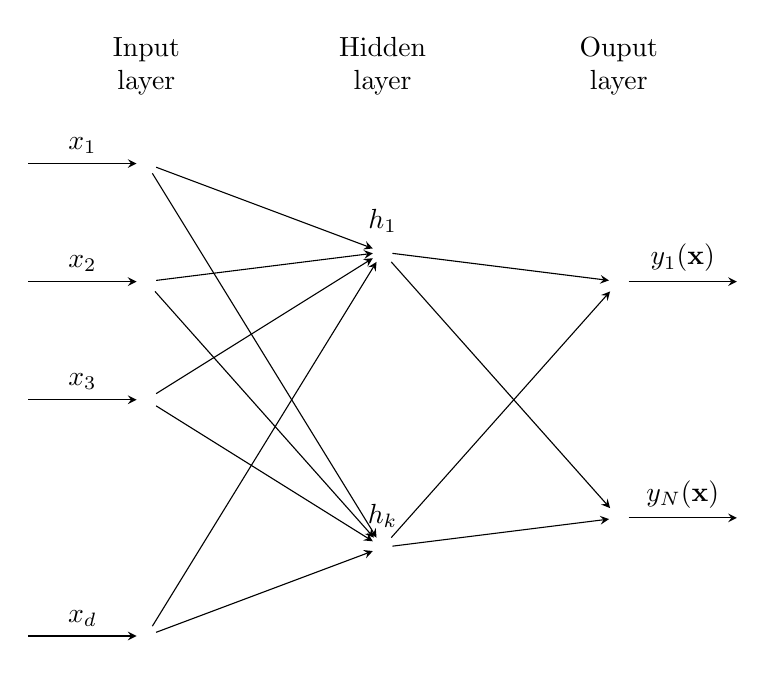
\begin{tikzpicture}[x=1.5cm, y=1.5cm, >=stealth]

% Create the input nodes
\foreach \m/\l [count=\y] in {1, 2, 3, missing, 4}
  \node [every neuron/.try, neuron \m/.try] (input-\m) at (0,2.5-\y) {};

% Create the hidden layer nodes
\foreach \m [count=\y] in {1, missing, 2}
  \node [every neuron/.try, neuron \m/.try ] (hidden-\m) at (2,2-\y*1.25) {};

% Create the output nodes
\foreach \m [count=\y] in {1, missing, 2}
  \node [every neuron/.try, neuron \m/.try ] (output-\m) at (4,1.5-\y) {};

% Label the input layer
\foreach \l [count=\i] in {1,2,3,d}
  \draw [<-] (input-\i) -- ++(-1,0)
    node [above, midway] {$x_\l$};

% Label the hidden layer
\foreach \l [count=\i] in {1,k}
  \node [above] at (hidden-\i.north) {$h_\l$};

% Label the output layer
\foreach \l [count=\i] in {1,N}
  \draw [->] (output-\i) -- ++(1,0)
    node [above, midway] {$y_\l(\mathbf{x})$};

% Connect the input layer to the hidden layer
\foreach \i in {1,...,4}
  \foreach \j in {1,...,2}
    \draw [->] (input-\i) -- (hidden-\j);

% Connect the hidden layer to the output layer
\foreach \i in {1,...,2}
  \foreach \j in {1,...,2}
    \draw [->] (hidden-\i) -- (output-\j);

\foreach \l [count=\x from 0] in {Input, Hidden, Ouput}
  \node [align=center, above] at (\x*2,2) {\l \\ layer};

\end{tikzpicture}

\end{document}
